%Capitulo 3, presentación 21
\definecolor{Pink}{RGB}{255,0,131}
\begin{frame}{Ejemplo: Juego del 8}
	\begin{columns}
		\begin{column}{0.5\textwidth}		
			\begin{figure}[h!]
				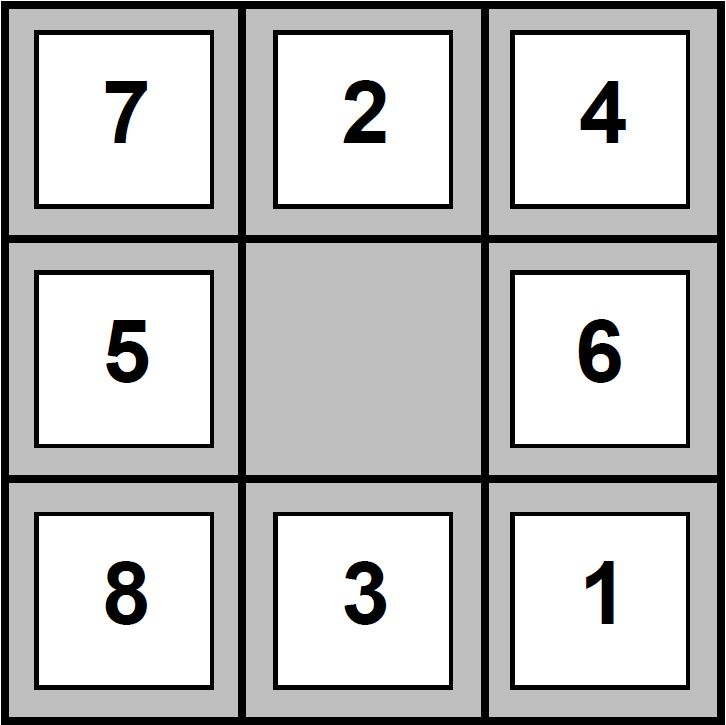
\includegraphics[scale=.15]{images/21_grid1.JPG}
				\\
				\vspace{0pt}
				{\tiny Estado Inicial}
			\end{figure}
		\end{column}
		
		\begin{column}{0.5\textwidth}  %%<--- here
			\begin{figure}
	     		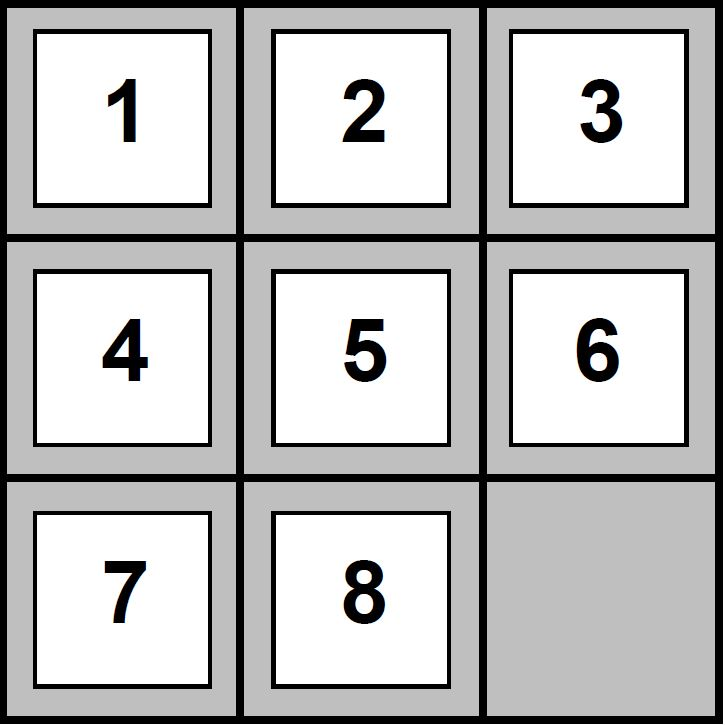
\includegraphics[scale=.15]{images/21_grid2.JPG}
	     		\\
				\vspace{0pt}
				{\tiny Estado Objetivo}
			\end{figure}
		\end{column}
	\end{columns}
	\vfill
	\small{	
            \textcolor{Pink}{\underline{¿Estados?}}: ubicaciones enteras de las casillas (ignorar posiciones intermedias)\\
            \textcolor{Pink}{\underline{¿Acciones?}}: mover a una casilla vacia a la izquierda, derecha, arriba, abajo (ignorar desajustes etc.)\\
            \textcolor{Pink}{\underline{¿Estado objetivo?}}\\
            \textcolor{Pink}{\underline{¿Costo de ruta?}}\\
    }
\end{frame}